% Compile with: lualatex sudoku.tex
\documentclass[11pt]{article}

\usepackage{amsmath, amssymb}
\usepackage{tikz}
\usepackage[a4paper, margin=2.5cm]{geometry}
\usepackage[colorlinks=true, urlcolor=blue]{hyperref}
\usepackage{fancyhdr}

\pagestyle{fancy}
\fancyhf{}
\renewcommand{\headrulewidth}{0pt}
\fancyfoot[L]{\small Junzhe Wang ~\textperiodcentered~
  \href{mailto:junzhe.wang2002@gmail.com}{\texttt{junzhe.wang2002@gmail.com}}}
\fancyfoot[R]{\small Last edited: \today\ ~\textperiodcentered~ p.\,\thepage}

\title{Sudoku}
\author{}
\date{}

\begin{document}

\maketitle
\thispagestyle{fancy}

\section{The puzzle and its rules}

A sudoku grid is a $9 \times 9$ board of cells, subdivided into nine
$3 \times 3$ \emph{boxes}. A puzzle starts with some cells filled in (the
\emph{givens}); the task is to fill every remaining cell with a digit from
$1$ to $9$ such that
\begin{itemize}
  \item every \textbf{row} contains each digit exactly once,
  \item every \textbf{column} contains each digit exactly once,
  \item every \textbf{box} contains each digit exactly once.
\end{itemize}
Each cell therefore belongs to three \emph{units} (its row, its column,
its box), and its 20 distinct \emph{peers} --- the other cells of those
units --- can never share its digit.

\begin{center}
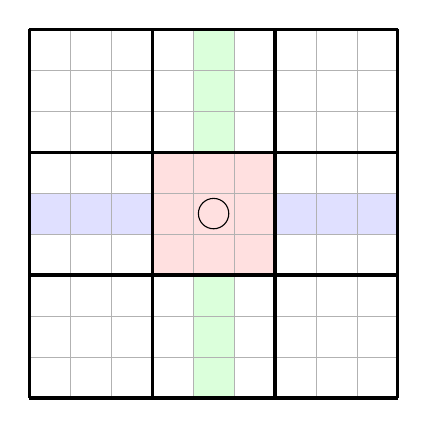
\begin{tikzpicture}[scale=0.52]
  \fill[blue!12] (0, 4) rectangle (9, 5);
  \fill[green!14] (4, 0) rectangle (5, 9);
  \fill[red!12] (3, 3) rectangle (6, 6);
  \draw[gray!60, very thin] (0, 0) grid (9, 9);
  \draw[very thick] (0, 0) grid[step=3] (9, 9);
  \node[circle, draw, inner sep=1pt] at (4.5, 4.5) {\phantom{0}};
\end{tikzpicture}

\smallskip
The three units of the circled cell: its row, its column, its box.
\end{center}

\section{Candidates and constraint propagation}

The solver's central data structure attaches to every empty cell its
\emph{candidate set}: the digits not yet ruled out. A digit placed in a
cell is erased from the candidates of all 20 peers. In the position below,
the circled cell sees $1, 7$ in its row, $3, 9$ in its column and $4, 5$
in its box, leaving candidates $\{2, 6, 8\}$ --- the small digits a
pencil-and-paper solver would write in the corner:

\begin{center}
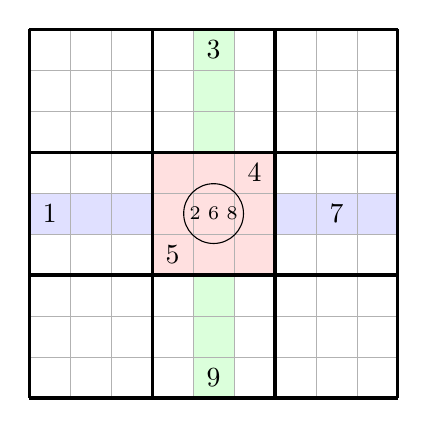
\begin{tikzpicture}[scale=0.52]
  \fill[blue!12] (0, 4) rectangle (9, 5);
  \fill[green!14] (4, 0) rectangle (5, 9);
  \fill[red!12] (3, 3) rectangle (6, 6);
  \draw[gray!60, very thin] (0, 0) grid (9, 9);
  \draw[very thick] (0, 0) grid[step=3] (9, 9);
  \node at (0.5, 4.5) {1};
  \node at (7.5, 4.5) {7};
  \node at (4.5, 8.5) {3};
  \node at (4.5, 0.5) {9};
  \node at (5.5, 5.5) {4};
  \node at (3.5, 3.5) {5};
  \node[circle, draw, inner sep=1.5pt] at (4.5, 4.5) {\scriptsize 2 6 8};
\end{tikzpicture}

\smallskip
Elimination: $\{1,\dots,9\}$ minus the row, column, and box gives
$\{2, 6, 8\}$.
\end{center}

Eliminations feed two deduction rules, and the rules feed further
eliminations:
\begin{itemize}
  \item \textbf{Naked single.} A cell whose candidate set shrinks to one
    digit must hold that digit. Placing it erases the digit from 20 more
    candidate sets --- which may create new singles.
  \item \textbf{Hidden single.} If, within one unit, some digit remains
    possible in only one cell, that cell must hold it --- even if the cell
    still has other candidates. Below, the digits $2, 4, 7$ are missing
    from the row; $4$ appears in only one candidate set, so it goes there:
\end{itemize}

\begin{center}
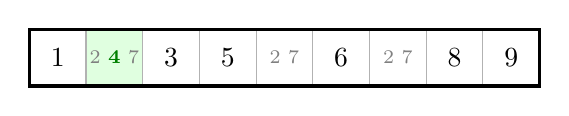
\begin{tikzpicture}[scale=0.72]
  \fill[green!12] (1, 0) rectangle (2, 1);
  \draw[gray!60] (0, 0) grid (9, 1);
  \draw[very thick] (0, 0) rectangle (9, 1);
  \node at (0.5, 0.5) {1};
  \node at (2.5, 0.5) {3};
  \node at (3.5, 0.5) {5};
  \node at (5.5, 0.5) {6};
  \node at (7.5, 0.5) {8};
  \node at (8.5, 0.5) {9};
  \node[font=\scriptsize, text=gray] at (1.5, 0.5)
    {2 \textcolor{green!50!black}{\textbf{4}} 7};
  \node[font=\scriptsize, text=gray] at (4.5, 0.5) {2 7};
  \node[font=\scriptsize, text=gray] at (6.5, 0.5) {2 7};
\end{tikzpicture}

\smallskip
A hidden single: of the three unresolved cells, only the shaded one still
has $4$ among its candidates.
\end{center}

Running eliminations and both rules until nothing changes is
\emph{constraint propagation} --- computing a fixpoint. Its power is easy
to underestimate: most published easy and medium puzzles dissolve
completely under propagation alone, with never a guess.

\section{Search: when logic stalls}

\paragraph{The stall.}
On hard puzzles propagation stalls short of a solution: a full pass over
all the rules changes nothing --- no elimination, no single --- yet some
cells still hold several candidates. The fixpoint has been reached, and it
is not yet the answer; the rules at hand are exhausted.

\paragraph{The remedy: guess and retract.}
Pick an unresolved cell, tentatively place one of its candidates, and
propagate as if the guess were fact. Two things can happen: either the
cascade rolls on --- sometimes all the way to a solution --- or it hits a
contradiction (a cell stripped of every candidate), which refutes the
guess; then rewind to the position before it and try the next candidate.
Here is the remedy at work on a stalled row:

\begin{center}
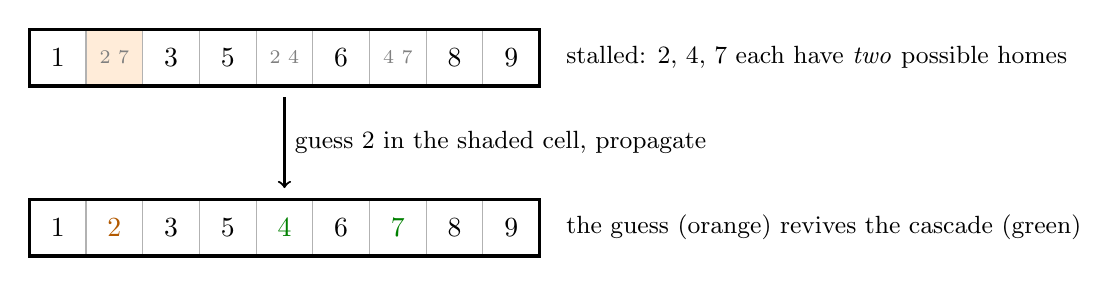
\begin{tikzpicture}[scale=0.72]
  % stalled row
  \fill[orange!15] (1, 3) rectangle (2, 4);
  \draw[gray!60] (0, 3) grid (9, 4);
  \draw[very thick] (0, 3) rectangle (9, 4);
  \node at (0.5, 3.5) {1};
  \node at (2.5, 3.5) {3};
  \node at (3.5, 3.5) {5};
  \node at (5.5, 3.5) {6};
  \node at (7.5, 3.5) {8};
  \node at (8.5, 3.5) {9};
  \node[font=\scriptsize, text=gray] at (1.5, 3.5) {2 7};
  \node[font=\scriptsize, text=gray] at (4.5, 3.5) {2 4};
  \node[font=\scriptsize, text=gray] at (6.5, 3.5) {4 7};
  \node[right, font=\small] at (9.3, 3.5)
    {stalled: $2$, $4$, $7$ each have \emph{two} possible homes};
  % the guess
  \draw[->, thick] (4.5, 2.8) -- (4.5, 1.2)
    node[midway, right, font=\small] {guess $2$ in the shaded cell, propagate};
  % resolved row
  \draw[gray!60] (0, 0) grid (9, 1);
  \draw[very thick] (0, 0) rectangle (9, 1);
  \node at (0.5, 0.5) {1};
  \node at (2.5, 0.5) {3};
  \node at (3.5, 0.5) {5};
  \node at (5.5, 0.5) {6};
  \node at (7.5, 0.5) {8};
  \node at (8.5, 0.5) {9};
  \node[orange!70!black] at (1.5, 0.5) {2};
  \node[green!50!black] at (4.5, 0.5) {4};
  \node[green!50!black] at (6.5, 0.5) {7};
  \node[right, font=\small] at (9.3, 0.5)
    {the guess (orange) revives the cascade (green)};
\end{tikzpicture}

\smallskip
\emph{Guessing $2$ leaves a naked single $4$; placing it leaves $7$.}
\end{center}

\paragraph{Guessing well.}
Recursing on guesses grows the familiar search tree of the earlier
quizzes; two refinements keep it tiny:

\begin{itemize}
  \item \textbf{Choose the most constrained cell} (fewest candidates
    remaining) --- the \emph{minimum remaining values} rule, \textbf{MRV}
    for short --- the same
    rescue-the-scarce principle as Warnsdorff's onward counts. A cell with
    two candidates gives a wrong guess a 50\% chance of instant
    refutation.
  \item \textbf{Propagate after every guess.} Each guess triggers the full
    cascade, so consequences surface immediately and contradictions
    appear after a handful of placements, not deep in the tree.
\end{itemize}

\section{Facts worth knowing}

\begin{itemize}
  \item \textbf{Uniqueness.} A \emph{proper} puzzle has exactly one
    solution; verifying properness means searching for a second solution
    and failing. A puzzle generator must run exactly that check on every
    candidate puzzle it digs out.
  \item \textbf{Seventeen givens.} No proper 9x9 puzzle with fewer than 17
    givens exists (McGuire, Tugemann and Civario, 2012 --- by exhaustive
    computer search), and 17-given puzzles do exist.
  \item \textbf{It scales badly, provably.} On generalized
    $n^2 \times n^2$ boards, sudoku is NP-complete; the 9x9 case is only
    tamed by its fixed size and by how sharply propagation prunes.
\end{itemize}

\section{From mathematics to program}

The program keeps the grid as 81 candidate sets (a solved cell is a
singleton) and implements propagation as the fixpoint of the two rules;
the solver wraps it in MRV-guided backtracking. The renderer draws what
solvers on paper actually do: pencil marks shrinking as eliminations
cascade, deduced digits appearing in one color, guesses in another, and a
contradiction flashing before its branch rewinds --- constraint
propagation made watchable.

\end{document}
